\chapter{Background}
In this section we will discuss the fundamentals of both model theory and neural networks. Since this thesis seeks to unify two vastly different fields of mathematics, understanding of both of them is essential. A reader acquainted with those fields should not find any surprises here.

%--------------------------------------------------------------

\section{Model theory}
Model theory is the area of mathematics that studies mathematical structures through the lens of mathematical logic.
\subsection{Basic definitions}
Most of these definitions are paraphrased from \cite{model}.
\begin{defn} A \textbf{language} $\mathcal{L}$ is a set of function, constant and relation symbols with associated arities.
\end{defn}

\begin{defn} A \textbf{term} in the language $\mathcal{L}$ is a finite sequence of function and constant symbols from $\mathcal{L}$ and variables that is defined recursively:
	\begin{enumerate}
	\item A variable is a term.
	\item A constant is a term.
	\item If $f$ is $n$-ary function and $t_1, \dots t_n$ are terms then $f(t_1, \dots t_n)$ is also a term.
	\end{enumerate}
Only sequences that can be obtained using this constructions are terms.
\end{defn}

\begin{defn} A \textbf{Formula} in the language $\mathcal{L}$ is a finite sequence of any symbols in $\mathcal{L}$, logical operations ($\wedge, \vee, \neg, \rightarrow$) and the equality symbol $=$. It is also defined recursively:
	\begin{enumerate}
		\item If $t_1$ and $t_2$ are terms then $t_1=t_2$ is a formula.
		\item If $R$ is an n-ary relation symbol and $t_1, \dots t_n$ are terms then $R(t_1, \dots t_n)$ is a formula. 
		\item If $\varphi$ is a formula then $\neg\varphi$ is also a formula.
		\item If $\phi$ and $\psi$ are formulas, then $\varphi\wedge\psi$, $\varphi\vee\psi$ and $\varphi\rightarrow\psi$ are also formulas.
	\end{enumerate}
	The definition usually also includes the quantifiers $\exists$ and $\forall$. 
	\begin{enumerate}
		\item[5.] If $\varphi$ is a formula and $x$ is a variable that is not already used with a quantifier then $(\exists x)\varphi$ and $(\forall x)\varphi$ are formulas.
		
		$\forall$ is called the \textit{universal} and $\exists$ is called the \textit{existential} quantifier
	\end{enumerate}
Once again, only sequences obtained by this construction are formulas. All subsequences of a formula that are also formulas are called \textbf{subformulas}.
\end{defn}

\begin{defn} Given a formula $\varphi$, a \textbf{free variable} is a variable in $\varphi$ that is not used in a quantifier. A variable that is used in a quantifier is called \textbf{bound}. If $x_1,\dots x_n$ are all the free variables of $\varphi$ then we usually write $\varphi$ as $\varphi(x_1,\dots x_n)$ to show that it has free variables.  A \textbf{sentence} is a formula that has no free variables. A \textbf{free formula} is a formula that has only free variables.
\end{defn}

\begin{defn}An \textbf{$\mathcal{L}$-theory} is a set of sentences in the language $\mathcal{L}$.
\end{defn}

Note that theory can be also infinite. Also note that the cardinality of a theory of a finite language is at most countable.

\begin{defn} A \textbf{structure} $\mathcal{S}$ is a collection $(S,\mathcal{I})$ where $S$ is a nonempty set (called the universe of $\mathcal{S}$) and $\mathcal{I}$ is an assignment that assigns interpretations to the elements of $\mathcal{L}$. Naturally it assigns function symbols to functions on $S$, constant symbols to elements of $S$ and relation symbols to relations on $S$ with their appropriate arities.
\end{defn}

Now we will need to know what does it mean for a sentence to be true in a structure. In order to do that we first need to know the values of terms.

\begin{defn}
Let $t(v_1\dots v_n)$ be an $\mathcal{L}$-term and $\phi:\{v_1,\dots v_n\}\longrightarrow S$ be an assignments of the variables to an $\mathcal{L}$-structure $\mathcal{S}$. Then we recursively assign values to subterms of $t$.
\begin{enumerate}
	\item Value of $v_i$ is $\phi(v_i)$
	\item Value of $c$ where $c$ is a constant is $\mathcal{I}(c)$
	\item If $t_1\dots t_m$ are terms with assigned values $s_1\dots s_m$ and $f$ is a function then $f(t_1,\dots t_m)$ is assigned the value $\mathcal{I}(f)(s_1,\dots s_m)$.
\end{enumerate}
\end{defn}

\begin{defn}
	Let $\varphi(x_1,\dots x_n)$ be an $\mathcal{L}$-formula and $\mathcal{S}$ an $\mathcal{L}$-structure. Then given a variable assignment $\phi:\{x_1,\dots x_n\}\longrightarrow S$ we assign the truth value of all subformulas of $\varphi$ as follows:
\begin{enumerate}
	\item If the subformula is of the form $t_1(x_1,\dots x_m)=t_2(x_1,\dots x_m)$ where $t_1$ and $t_2$ are terms, then it is true if and only if $t_1$ and $t_2$ have the same value assigned with variable assignment $\phi$.
	\item If the subformula is of the form $R(t_1, \dots t_r)$ where $t_1, \dots t_r$ are terms with assigned values $s_1, \dots s_r)$ then it is true if and only if $\mathcal{I}(R)(s_1,\dots s_r)$ holds in $\mathcal{S}$.
	\item Any logical operators work as normal, e.g. $\neg \psi$ is true if and only if $\psi$ is false or $\psi_1 \wedge \psi_2$ is true if and only if both $\psi_1$ and $\psi_2$ are true in this assignment. 
	\item If the subformula is of the form $(\forall y) \psi(y,x_1,\dots x_m)$ then it is true if and only if for any extension $\phi'$ of $\phi$ that includes also assigns $y$ does $\psi(y,x_1,\dots x_m)$ hold (with assignment $\phi'$).
	
	Alternatively if the subformula is of the form $(\exists y)\psi(y,x_1,\dots x_m)$ then we only require that there exists at least one such $\phi'$.
\end{enumerate}
\end{defn}

\begin{defn}
Given an $\mathcal{L}$-formula $\varphi(x_1,\cdots x_n)$ we say that $\varphi$ \textbf{holds} in an $\mathcal{L}$-structure $\mathcal{S}$ if it is true for any variable assignment. We denote $\mathcal{S}\models \varphi(x_1,\dots x_n)$. A formula $\varphi$ is satisfiable if there exists a structure $\mathcal{S}$ in the same language where $\mathcal{S}\models \varphi$
\end{defn}
Note that this definition also works if $\varphi$ is a sentence.

\begin{defn}
Given an $\mathcal{L}$-theory $T$, we say that an $\mathcal{L}$-structure $\mathcal{S}$ is a \textbf{model} of $T$ if $T\models \varphi$ for every $\varphi\in T$.
\end{defn}

\begin{defn}
Formulas $\varphi$ and $\psi$ are \textbf{equivalent} if they are both true under the same variable assignments of their free variables in any of their models\footnote{This definition is not the standard one, since we only define equivalence with respect to models. Normally equivalence of formulas is a semantic property, regardless of models or even satisfiability. However, to define equivalence properly, we would need to define multiple other terms from mathematical logic, which we will not do for better readability of this section. Classic definition can be found in \cite{logic}.}.
\end{defn}
This $\mathcal{S}$ is by no means unique. In fact, most theories have vastly different models.

Note that this definition does not include semantic differences, e.g. renaming of variables. For this we use a different definition:

\begin{defn}
	We say that $\mathcal{L}$-formulas $\varphi$ and $\psi$ are \textbf{equisatistfiable} if either both are satisfiable or both are not.
\end{defn}

The models of $\varphi$ and $\psi$ can be different, they might not even be in the same language. Every double of equivalent formulas is also equisatisfiable, since they share all models \footnote{This is also true with the classical definition of equivalence, even though it does not require the formulas to be satisfiable.}. This term is used almost exclusively in formula manipulations.

Important things to notice in this section are that the universe $S$ has no restrictions. Here we will use $S$ as a subset of $\mathbb{R}^n$ in order to allow working with neural networks. 

\subsection{Skolemization}
The existence of existence quantifiers has been a major hurdle for automatic theorem provers to overcome, since it adds a lot of complexity to the proving algorithm. For example if a formula starts with $\forall x \exists y \forall z$ then $y$ can be completely different for each $x$, but does not depend on $z$. To "remember" this dependency in further proofs, the theorem prover needs to do some processing. We call this process \textbf{Skolemization} by it's inventor, Thoralf Skolem.

\begin{defn}
	We say that a formula $\varphi$ is in \textbf{prenex normal form} if it is written as a sequence of quantifiers followed by a free formula.
\end{defn}

\begin{thm}
	Every formula is equivalent to a formula in prenex normal form.
\end{thm}
\begin{proof}
	We recursively apply the quantifier equivalence rules (we also assume that there exists at least one element):
	\begin{itemize}
		\item $(Q x\ \varphi)\wedge\psi$ is equivalent to $Q x\ (\varphi\wedge\psi)$ where $Q$ is either $\exists$ or $\forall$. 
		\item $(Q x\ \varphi)\vee\psi$ is equivalent to $Q x\ (\varphi\vee\psi)$ where $Q$ is either $\exists$ or $\forall$. 
		\item $\neg(\exists x\varphi)$ is equivalent to $\forall x \neg \varphi$
		\item $\neg(\forall x\varphi)$ is equivalent to $\exists x \neg \varphi$
	\end{itemize}
If we treat implication $\varphi \rightarrow \psi$ as equivalent to $\neg \varphi \vee \psi$ we are done.
\end{proof}

\begin{defn}
	We say that a formula $\varphi$ is in \textbf{Skolem normal form} if it is in prenex normal form and all quantifiers are universal.
\end{defn}

Skolemization is a process that turns formulas from prenex normal forms to Skolem normal form by introducing new function and constant symbols. We repeatedly apply this step:

Let $\varphi$ be a formula that has the form $$\forall x_1\forall x_2,\dots \forall x_{i}\exists y\psi(x_1,\dots x_i,y)$$ where $x_1,\dots x_n$ are all universally quantified and $\psi$ is a formula in prenex normal form. Then Skolemized version of $\varphi$ is obtained by introducing a new $i$-ary function symbol $f_y$ and replacing all occurences of $y$ in $\psi$ with $f_y(x_1,\dots,x_i)$. Thus we get $$\forall x_1\forall x_2,\dots \forall x_{i}\psi(x_1,\dots x_i,f_y(x_1,\dots,x_i))$$ We say that $f_y$ is the Skolem function of $y$.

If $\varphi$ has the form $\exists y \psi(y)$, i.e. there are no universal quantifiers at the start we introduce a Skolem constant $c_y$ and replace all occurences of $y$ in $\psi$ by $c_y$, obtaining $\psi(c_y)$. This is consistent with the notion of constants being $0$-ary functions.

\begin{thm}
	Every formula $\varphi$ is equisatisfiable to the formula $\phi$ that is obtained by the Skolemization process.
\end{thm}
\begin{proof}
	We need to prove that we can build a model of $\phi$ from a model of $\varphi$ and vice versa. Let $\mathcal{S}$ be a model of $\varphi$ and WLOG let $\varphi$ be in prenex normal form $Q_1x_1,\dots Q_nx_n\psi(x_1,\dots x_n)$ where $Q$-s are quantifiers and $\psi$ is a free formula. We need to add interpretations of all Skolem functions and constants to build the model $\mathcal{S}'\models\phi$. 
	
First, let us assume that $y$ is the first existentially quantified variable in $\varphi$ and $f_y(x_1,\dots,x_i)$ its Skolem function (to include Skolem constants we permit $i=0$). Since $\mathcal{S}$ is a model of $\varphi$, we know that for every $x_1,\dots x_i\in S$ there exists an $y$ that is the "witness" that $\varphi$ holds. We define $f_y(x_1,\dots x_i)=y$. Since there is such $y$ for every tuple of $x$-es, this is a well-defined function. And we can easily see, $\psi(x_1,\dots x_i,y,x_{i+2},\dots x_n)$ has the same truth value in $\mathcal{S}$ as $\psi(x_1,\dots x_i,f_y(x_1,\dots x_i),x_{i+2},\dots x_n)$ does in $\mathcal{S}'$, therefore $\mathcal{S}'\models\phi$. We repeat this process of defining Skolem functions for every step of the Skolemization process, and we get the whole $\mathcal{S}'$.

The other way around is just as easy. Since $\psi(x_1,\dots x_i,f_y(x_1,\dots x_i), x_{i+1},\dots,x_n)$ holds in $\mathcal{S}'$, there obviously exists an $y\in S$ that $\psi(x_1,\dots x_i,y, x_{i+1},\dots,x_n)$, that being $y=f_y(x_1,\dots x_i)$.
\end{proof}

This process had first been introduced to prove a general theorem in model theory, but we will use it to enable manipulation with existential quantifiers. More about the usage of this theorem can be found in \cite{logic} and \cite{model}.

\subsection{Substructures and extensions}
\label{section:extensions}

In order to do any constructions in model theory, we need to know how models relate to each other. As it is right now, our models exist completely separate from each other, with the only comparisons being possible through the lens of formulas. However, if two structures are models of the same theory, we can not differentiate between them using just that theory. That is why we need the notions of substructures and extensions.

\begin{defn}
	Let $\mathcal{S},\mathcal{T}$ be structures in the same language $\mathcal{L}$. Then a \textbf{mapping} of $\mathcal{S}$ to $\mathcal{T}$ is any function $f:S\rightarrow T$ that satisfies the following (for any $x_1,..,x_n\in S$):
	\begin{enumerate}
		\item If $F$ is an $n$-ary function in $\mathcal{L}$ then $f(F_\mathcal{S}(x_1,\dots,x_n))=F_\mathcal{T}(f(x_1),\dots,f(x_n))$.
		\item If $c$ is a constant in $\mathcal{L}$ then $f(c_\mathcal{S})=c_\mathcal{T}$.
		\item If $R$ is an $n$-ary relation in $\mathcal{L}$ then $R_\mathcal{S}(x_1,\dots,x_n)$ holds if and only if $R_\mathcal{T}(f(x_1),\dots,f(x_n))$ holds.
	\end{enumerate}
If also holds that $f$ is one-to-one, then $f$ is called an \textbf{embedding}.
\end{defn}

\begin{defn}
	We say that a structure $\mathcal{S}$ is a \textbf{substructure} of $\mathcal{S}'$ if they are in the same language, $S\subseteq S'$ and all symbol interpretations agree on $S$. That means that $(S,\left.\mathcal{I}\right|_S)$ is a structure. Here $\left.\mathcal{I}\right|_S$ means the assignments of symbols is the same but restricted to $S$.
	
	We also say that $\mathcal{S}'$ is an \textbf{extension} of $\mathcal{S}$
\end{defn}

There are not many things that hold in extensions for general. For example a carthesian product of two structures with naturally defined functions, constants and relations is an extension of both of them, but their elements do not necessarily "interact" with each other. To ensure this interaction we need new definitions.

\begin{defn}
	Let $\mathcal{S}$ be an $\mathcal{L}$-structure and $\mathcal{S}'$ its extension.  Let $t_1(x)$ and $t_2(x)$ be $\mathcal{L}'$-terms with only one variable where $\mathcal{L}'$ is the language $\mathcal{L}$ with added names for each element of $S$. We say that the predicate\footnote{Predicate is a formula with only one free variable} $\varphi(x): "t_1(x)=t_2(x)"$ is an \textbf{equation} in $\mathcal{S}$. If $\varphi(x)$ holds for some $x$, we say that that $x$ is the \textbf{solution} of $\varphi$. If the set of solutions of $\varphi$ is not $S$, we say that the equation is \textbf{non-zero}.
\end{defn}
\begin{defn}	
	Let $s\in S'$ be an element. If is there exists a non-zero equation $\varphi(x)$ in $\mathcal{S}$ for which $s$ is a solution then $s$ is \textbf{algebraic}\footnote{Normally we do not require the $\varphi$ to be an equation, but for the purposes of our model we will make this assumption}. If there is no such equation, then $s$ is \textbf{transcendental}.
\end{defn}

We see that every element $s\in S$ is algebraic. We can take $x=s$ as the equation.

A reader acquainted with field extensions will recognize these terms. Indeed, these are generalizations of those terms, so that the theory can be modified and applied to other structures than fields. A crucial difference is that this definition does not guarantee the existence of an extension. An example of this is $0\cdot x=1\cdot x$ in any field. However, there are classes of structures where every equation yields an algebraic extension. One such example are groups.

\subsection{Groups and their algebraic extensions}
\label{section:groups}

\begin{defn}
A \textbf{group} is a structure in the language $\{\cdot,^{-1},e\}$ (where $\cdot$ is binary function, $^{-1}$ is unary and $e$ is a constant) that also models the following theory\footnote{For the sake of simplicity we will use multiple $=$ signs in the definitions. To be absolutely correct, we could re-write these as $a=b=c \longrightarrow a=b\wedge b=c \wedge c=a$.}
\begin{enumerate}
	\item $\forall a,b,c\ (a\cdot b)\cdot c = a \cdot (b\cdot c)$
	\item $\forall a\ a\cdot e = e\cdot a = a$
	\item $\forall a\ a\cdot a^{-1}=a^{-1}a=e$
\end{enumerate}
We will call $\cdot$ \textbf{composition}, $^{-1}$ \textbf{inverse} and $e$ shall be \textbf{unit}.
\end{defn}

Note that this is the skolemized version of the theory that has $\exists e \forall a\ e\cdot a = a\cdot e = a$ or $\exists e(\forall a\ e\cdot a = a\cdot e = a \wedge\forall a \exists b\ a\cdot b = b\cdot a = e)$\footnote{Once again we use simplified notation.}. 

\begin{defn}
	A substructure of a group is a \textbf{subgroup} (denoted $G\leq G'$). We say that a subgroup is \textbf{normal} if $\forall x\in G'\ \forall g\in G\ x^{-1}\cdot g\cdot x\in G$, or simply $x^{-1}Gx\leq G$. We denote it as $G\trianglelefteq G'$.
\end{defn}

It can be proven that this subgroup is of the form $\{t(b_1,\dots b_n)|b_1,\dots b_n\in B, t \text{ is a term}\}$. It is also the intersection of all groups that contain $B$ (\cite{group}). Note that if we use this as a definition, we can expand the notion of a generated substructure to any model.

\begin{defn}
	Let $G$ be a group and $B$ a set of elements of $G$. Then a subgroup \textbf{generated} by $B$ is the smallest subgroup of $G$ that contains $B$. We denote it as $\langle B\rangle_G$.
\end{defn}

\begin{defn}
	Let $G\leq H$ be two groups. Then the sets $hG=\{h\cdot g|g\in G\}$ for any $ h\in H$ are called  \textbf{left cosets} of $G$. If $G$ is a normal subgroup, then we can induce a composition on these cosets: $hG\cdot h'G=(h\cdot h')G$ (a proof that this is really a group can be found in \cite{group}). We will call this group the \textbf{quotient group} $H/G$.
\end{defn}

As with algebraic extensions over fields, we can use this quotient group to craft an algebraic extension to any equation.

First, however, we need a group that we can do quotient of.

\begin{defn}
\label{freegroupdefn}
	Let $G$ be a group. Then we will define an extension $G[x]$ as such:
	\begin{itemize}
		\item Elements of $G[x]$ are formal strings of the form $g_1 x^{n_1}g_2 x^{n_2}\dots g_k x^{n_k}g_{k+1}$ where $k$ can be any integer (including $0$-in that case we have an element of $g$), $g_i$ are elements of $G$ (all except $g_1$ and $g_{k+1}$ have to be different from $e$) and $n_i$ are non-zero integers.
		\item $\cdot$ is defined as concatenation of strings with adjustment for inverses. We do this adjustment by repeating the following:
			\begin{enumerate}
				\item If we there is a substring $g_i g_{i+1}$ we replace it with $(g_i\cdot g_{i+1})$.
				\item If there is a substring $x^{n_{i-1}}ex^{n_i}$ we replace it by $x^{n_{i-1}+n_i}$.
				\item If there is $x^0$, we replace it by $e$.			
			\end{enumerate}
			If none of these replacements is possible, we have a valid element.
	\item $e$ is the same as in $G$.
	\item If  $g=g_1 x^{n_1}g_2 x^{n_2}\dots g_k x^{n_k}g_{k+1}$ then $g^{-1}=g_{k+1}^{-1}x^{-n_k}\dots x^{-n_1}g_1^{-1}$. We can easily verify that $g\cdot g^{-1}$ is indeed equal to $e$.
	\end{itemize}
\end{defn}

Without loss of generality we can assume that any equation $\varphi$ has the form $t(x)=e$, where $t$ is a term. If $\varphi(x): "t_1(x)=t_2(x)"$ would have a different form, then $\varphi'(x): "t_1(x)\cdot (t_2(x))^{-1}=e"$ has exactly the same solutions.

\begin{thm}
	Let $G$ be a group and $\varphi(x)$ an equation of the form $t(x)=e$ where $t(x)$ has at least one occurence of $x$. Then there exists an extension $G'$ of $G$ such that there exists $g\in G'$ that is a solution to $\varphi$.
\end{thm}
\begin{proof}
If we apply simplifications from definition \autoref{freegroupdefn}, $t$ has the form $g_1 x^{n_1}g_2 x^{n_2}\dots g_k x^{n_k}g_{k+1}$. This modification of $\varphi$ still has the same solutions.

This way $t$ can be seen as an element of $G[x]$. Let us then define $B=\{gtg^{-1}|g\in G[x]\}$. $\langle B\rangle$ is a normal subgroup of $G[x]$. We immediately see that $gbg^{-1}\in \langle B\rangle$, (even $gbg^{-1}\in B$) for all $b\in B, g\in G[x]$. Now if $b=b_1 b_2\dots b_n$ where $b_i\in B$ then $$gbg^{-1}=gb_1 b_2\dots b_ng^{-1}=gb_1g^{-1}g b_2g^{-1}\dots gb_ng^{-1}.$$
We define ${b_i}'=gb_ig^{-1}$ for $i\in\{1,\dots,n\}$. Now $$gbg^{-1}=(gb_1g^{-1})(g b_2g^{-1})\dots (gb_ng^{-1})={b_1}'{b_2}'\dots{b_n}'.$$
Since $\forall i\ {b_i}'\in B$, also $gbg^{-1}\in \langle B\rangle$.

Now we know that $G[x]/\langle B \rangle$ is a group. In it, all elements of $G$ form different cosets, since $g\langle B \rangle$ always has the element $g\cdot t(x)$ and no two $g\in G$ can produce the same $g\cdot t(x)$. Also, since $t(x)$ has at least one occurence of $x$, we know that $g\notin \langle B \rangle\ \forall g\in G$. Therefore $G\leq G[x]/\langle B \rangle$.

The last thing we need to show is that $x \langle B \rangle$ is a solution to $\varphi(x)$. Indeed, since $t(x)\in\langle B \rangle$, $$t(x\langle B \rangle)=t(x)\langle B \rangle=\langle B \rangle=e_{G[x]/\langle B \rangle}.$$

Therefore $G[x]/\langle B \rangle$ is the desired extension.
\end{proof}

A reader acquainted with field extensions will immediately recognize this construction. Indeed, it had been the inspiration for this proof. Worth noticing is that this construction can also naturally lead to the notions of Galois groups and indices of group extensions, but that is beyond the scope of this thesis.

In order to describe some of the extensions of groups that are obtained in this thesis, we need a new type of construction: a \textbf{semidirect product}. There are two different versions of this construction, we will use the so-called outer one.

\begin{defn}
	Let $H,K$ be groups and $\varphi:K\rightarrow \text{Aut}(H)$\footnote{For the definition of homomorphisms and automorphisms of groups, refer to \cite{group}. In short, a homomorphism is a mapping $f:G\rightarrow H$ such that $f(g_1g_2)=f(g_1)f(g_2)$ and automorphism is an invertible homomorphism $G\rightarrow G$.} a homomorphism (for the sake of clarity we will refer to $\varphi(k)$ as $\varphi_k$). Then the semidirect product $H \rtimes_{\varphi} K$ is defined as such:
	\begin{itemize}
		\item Universe is the set $H\times K$.	
		\item $(h_1,k_1)\cdot(h_2,k_2)$ is defined as $(h_1\varphi_{k_1}(h_2),k_1k_2)$
		\item $(h,k)^{-1}$ is defined as $(\varphi_k^{-1}(h^{-1}),k^{-1})$
		\item $e=(e_H,e_K)$
	\end{itemize}
\end{defn}
Proof that this is indeed a group can be found in \cite{group}.
%-------------------------------------------------------
%-------------------------------------------------------
%-------------------------------------------------------
%-------------------------------------------------------

\section{Neural networks}
Neural networks have been one of the most important and well developed methods in machine learning in recent years. The main advantage of their usage is their universal property - the fact that given an $\epsilon>0$ there exists for every smooth function a neural network that approximates it with the error of at most $\epsilon$. Assuming that we have a structure whose universe is a subset of $\mathbb{R}^n$, we can approximate any of its functions with arbitrary precision. How exactly do we do that will be discussed in \autoref{chapter:implementation}. More about this subject can be found in \cite{neural}. This publication is also the principal source for this section.

\subsection{What is a neural network}
In this section we will describe a \textbf{feedforward neural network}. We call it feedforward because it lacks feedback connections. It is therefore simpler, although it does not have any "memory". If a network has feedback connections, it is called \textbf{recurrent}. They are also widely used in machine learning, they are not used here, thus are beyond the scope of this thesis.

A network is usually represented by chaining of functions, called \textbf{layers}. Thus if we have a network $f(x)=f_n(f_{n-1}(\dots f_1(x))\dots)$ we call $f_1$ the first layer, $f_2$ second and so on. The number of these layers is called \textbf{depth} of a model. The last layer is called \textbf{output layer}, while the rest are called \textbf{hidden layers} since we usually can not interpret what does the data they are using mean.

In general the output $f_i$ does not need to have the same dimension as the input $x$ or the output $y$. But for the sake of simplicity, all hidden layers usually tend to have the same dimension between them. This is called the \textbf{width} of the network. Both depth and width can have a profound effect on the network's performance. 

These networks are called neural, because they are inspired by biological neurons. In each layer the singular neurons are scalar functions from each element of input to each element of the output. These elements are also commonly referred to as \textit{nodes}. When we add together all neurons that lead to a node of the output, we get a vector to scalar function, that is the building block of a layer. This is better illustrated in \autoref{nndiagram1}.

\begin{figure}[h]
\center
\caption{Neurons in a layer}
\label{nndiagram1}
\medskip
\begin{tikzpicture}[circ/.style={circle,draw,minimum size=1em}]
\foreach \i in {4,...,1}
{
	\node[circ](a\i)at(-1,\i){};
	\node[circ](b\i)at(1,\i){};
}
\foreach \i in {1,...,4}
{
	\draw[->,-latex'](a\i)--(b4);
	\draw[->,-latex'](a\i)--(b3);
}
\node[] at (0,6){\small{Each arrow represents a single neuron-a scalar to scalar function}};
\end{tikzpicture}
\end{figure}	

The simplest neural networks are linear models, e.g. linear regression. In these models each neuron is a simple multiplication by a parameter. These models   however have many drawbacks, for instance that they can only model linear functions. That is because the layers are linear functions, therefore several layers in a sequence also form a linear function.

We overcome this by altering the layer input in a non-linear fashion, ideally preserving the most important parts of it. This is an important area of ongoing research.

One of the most widely used methods to break the linearity is the use of so-called activation functions. Activation function is a non-linear $\mathbb{R}\rightarrow \mathbb{R}$ function that we perform on each node to know if it "activates". There are several functions that fulfill this purpose, each with their advantages and disadvantages. The simplest is $ReLU$: the \textbf{Re}ctified \textbf{L}inear \textbf{U}nit (\cite{relu1}, \cite{relu2}, \cite{relu3}). It is defined as $ReLU(x)=max\{x,0\}$. It is the most used activation function because it is the simplest function that also preserves most of what makes linear functions easy to work with (simple derivation). It has however some drawbacks that we will discuss later.

\begin{figure}[h]
\caption{ReLU}
\center
\begin{tikzpicture}
	\draw[->](-3,0)--(3,0)node[midway,anchor=north]{$0$}node[below]{$x$};
	\draw[->](-3,0)--(-3,5)node[midway,anchor=east]{$y$};
	\draw[dotted](0,0)--(0,1);
	\node[anchor=east] at (-3,1){$0$};
	\draw[line width=2] (-3,1)--(0,1)--(3,4);
\end{tikzpicture}
\end{figure}

\subsection{Example: XOR}

One of the simplest examples of the usefulness of this non-linearity is the binary operation XOR: the e\textbf{X}clusive \textbf{OR}. It is a function $\{0,1\}^2\rightarrow \{0,1\}$ that is $1$ if and only if exactly one of the inputs is $1$. This function is impossible to approximate with linear regression, but there exists a simple network with $ReLU$ activation functions that exactly approximates it. This example network is the same as can be found in \cite{neural}.

Let us start with linear regression. As the loss function we will use the most common one, mean square error. It has the form
$$J(\theta)=\frac{1}{n}\sum(\widehat{f}(\textbf{x};\theta)-f(\textbf{x}))^2$$
where $f$ is the function we try to estimate and $\widehat{f}$ is the learned function. Since we are now using linear regression, $\widehat{f}$ has the form $\widehat{f}(\textbf{x};\textbf{w},b)=\textbf{x}^\top \textbf{w}+b$ where $\textbf{w}$ is called the weight vector and $b$ is bias (in this case scalar). Using the least squares method we get $\textbf{w}=(0,0)^\top$ and $b=\frac{1}{2}$. This is obviously not a good fit as it just outputs $\frac{1}{2}$ regardless of the input.

If we however permit the usage of activation functions (ReLU), we can handcraft a network that will fit the function perfectly. Now our network will have the form 
$$\widehat{f}(\textbf{x};\textbf{W},\textbf{c},\textbf{w},b)=\textbf{w}^\top \max\{0,\textbf{W}^\top\textbf{x}+\textbf{c}\}+b$$ 
where 
$$\textbf{W}=
\left(\begin{matrix}
	1 & 1\\
	1 & 1
\end{matrix}\right),$$
$$\textbf{c}=
\left(\begin{matrix}
	0\\
	-1
\end{matrix}\right),$$
$$\textbf{w}=
\left(\begin{matrix}
	1\\
	-2
\end{matrix}\right),$$
and $b=0$. This network is illustrated in \autoref{xordiagram}. This is also not the only network that estimates XOR perfectly.
\begin{figure}[h]
\caption{XOR network}
\center
\label{xordiagram}
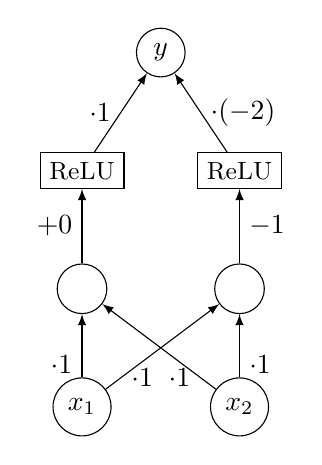
\begin{tikzpicture}
	\node[circle,draw](in1) at (0,0){$x_1$};
	\node[circle,draw](in2) at (2,0){$x_2$};
	\node[circle,draw](mid1) at (0,1.5){$\ \ \ $};
	\node[rectangle,draw](relu1) at (0,3){\small{ReLU}}; 
	\node[circle,draw](mid2) at (2,1.5){$\ \ \ $};
	\node[rectangle,draw](relu2) at (2,3){\small{ReLU}}; 
	\node[circle,draw](out) at (1,4.5){$y$};
	\draw[-latex](in1)--(mid1) node[pos=0.2,anchor=east]{$\cdot 1$};
	\draw[-latex](in1)--(mid2) node[pos=0.14,anchor=west]{$\cdot 1$};
	\draw[-latex](in2)--(mid1) node[pos=0.14,anchor=east]{$\cdot 1$};
	\draw[-latex](in2)--(mid2) node[pos=0.2,anchor=west]{$\cdot 1$};
	\draw[-latex](mid1)--(relu1) node[midway,anchor=east]{$+0$};
	\draw[-latex](mid2)--(relu2) node[midway,anchor=west]{$-1$};
	\draw[-latex](relu1)--(out) node[midway,anchor=east]{$\cdot 1$};
	\draw[-latex](relu2)--(out) node[midway,anchor=west]{$\cdot (-2)$};
	
\end{tikzpicture}
\end{figure}

Let us see what happens when we apply the input data to it in matrix form $$
\left(\begin{matrix}
	0 & 0\\
	1 & 0\\
	0 & 1\\
	1 & 1
\end{matrix}\right).$$
After the first layer multiplication by the weight matrix $\textbf{W}$ we have
$$\left(\begin{matrix}
	0 & 0\\
	1 & 1\\
	1 & 1\\
	2 & 2
\end{matrix}\right).$$

When we add the bias vector $\textbf{c}$ we get 
$$
\left(\begin{matrix}
	0 & -1\\
	1 & 0\\
	1 & 0\\
	2 & 1
\end{matrix}\right).$$

Now we apply ReLU:
$$
\left(\begin{matrix}
	0 & 0\\
	1 & 0\\
	1 & 0\\
	2 & 1
\end{matrix}\right).$$

This concludes the first layer of the network. Then we multiply each row with $\textbf{w}^\top$ and we get
$$	
\left(\begin{matrix}
	0\\
	1\\
	1\\
	0
\end{matrix}\right)$$
which is exactly the desired output.

In this case we got the hand-crafted solution from a book. Normally the weights and biases are found using an optimization method such as gradient descent. Here we found the perfect solution, a global minimum to the loss function. But that is not generally possible.

\subsection{Other activation functions}
ReLU, while being the most popular activation function, is not the only one used here, because it also has some drawbacks. The fact that its gradient is $0$ on all negative inputs means that gradient descent optimization methods might get us to the state where a node "dies" - all gradients regardless of data are 0. This tends to happen if our input and output contain few non-zero elements. In that case it is advised to use a different activation function.

Before the introduction of ReLU the default activation functions were sigmoid $$\sigma(x)=\frac{1}{1+e^{-x}}$$ and hyperbolic tangent $$\tanh(x)=\frac{e^x-e^{-x}}{e^x+e^{-x}}$$ functions. They are related to each other since $\tanh(x)=2\sigma(2x)-1$. The main advantage of these functions is that they only output values in an open interval, $(0,1)$ for sigmoid and $(-1,1)$ for tanh. They also have nonzero gradient over their whole domain, which ensures that gradient descent optimization always works. However, as can be seen in \autoref{sigmoiddiagram} if the inputs are far enough from $0$, the gradients become very small. This results in gradient descent optimizers taking longer time (\cite{imagenet_relu}). If this happens, we say that the functions \textbf{saturate}. This is also the reason why these functions fell out of use.
\begin{figure}[t]
\caption{Sigmoid and tanh functions}
\center
\label{sigmoiddiagram}
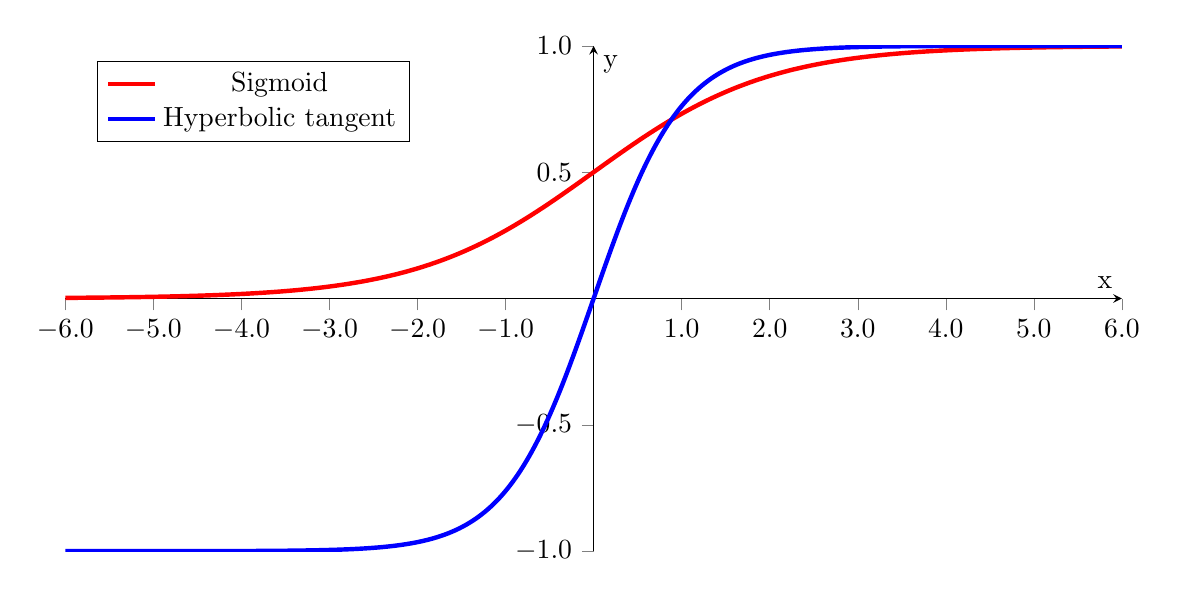
\begin{tikzpicture}
    \begin{axis}[
    	legend pos=north west,
        axis x line=middle,
        axis y line=middle,
        x tick label style={/pgf/number format/fixed,
                            /pgf/number format/fixed zerofill,
                            /pgf/number format/precision=1},
        y tick label style={/pgf/number format/fixed,
                            /pgf/number format/fixed zerofill,
                            /pgf/number format/precision=1},
        width=15cm,
        height=8cm,
        xmin=-6,     % start the diagram at this x-coordinate
        xmax= 6,    % end   the diagram at this x-coordinate
        ymin= -1,     % start the diagram at this y-coordinate
        ymax= 1,   % end   the diagram at this y-coordinate
        %axis background/.style={fill=white},
        xlabel=x,
        ylabel=y,
        tick align=outside,
        enlargelimits=false]
      % plot the stirling-formulae
      \addplot[domain=-6:6, red, ultra thick,samples=500] {1/(1+exp(-x))};
      \addplot[domain=-6:6, blue, ultra thick, samples=500]{tanh(x)};
      \addlegendentry{Sigmoid}
      \addlegendentry{Hyperbolic tangent}
    \end{axis}
\end{tikzpicture}
\end{figure}

\begin{figure}[h]
\caption{ReLU variations}
\center
\label{variousreludiagram}
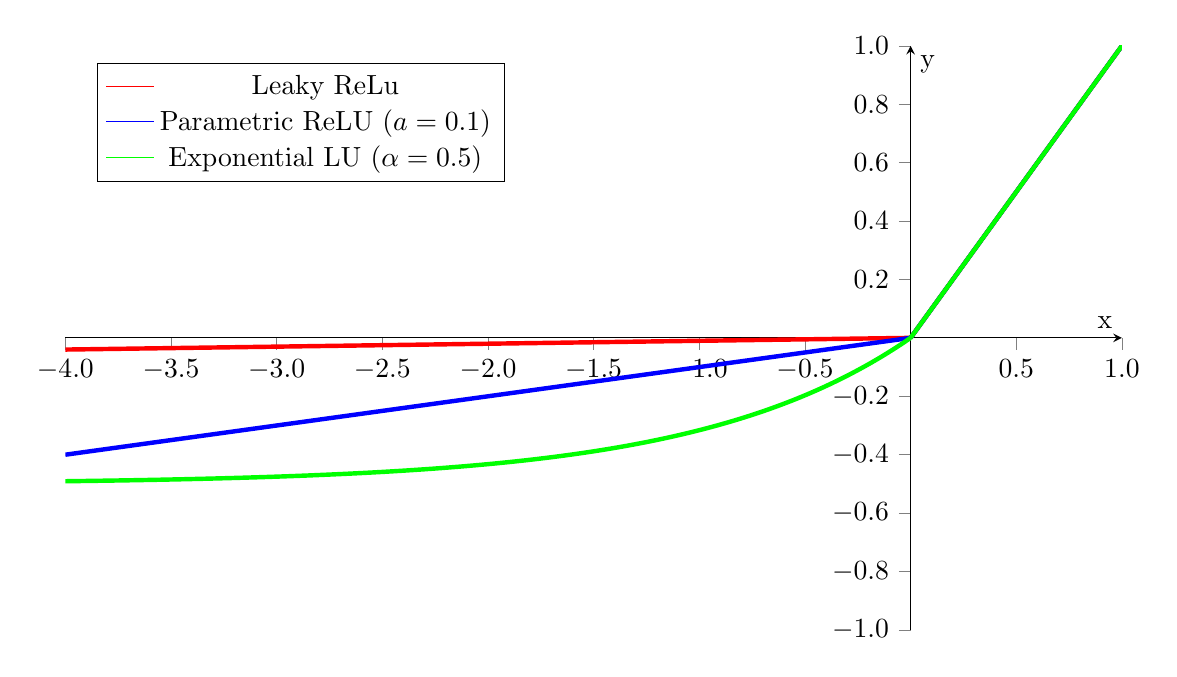
\begin{tikzpicture}
    \begin{axis}[
    	legend pos=north west,
        axis x line=middle,
        axis y line=middle,
        x tick label style={/pgf/number format/fixed,
                            /pgf/number format/fixed zerofill,
                            /pgf/number format/precision=1},
        y tick label style={/pgf/number format/fixed,
                            /pgf/number format/fixed zerofill,
                            /pgf/number format/precision=1},
        width=15cm,
        height=9cm,
        xmin=-4,     % start the diagram at this x-coordinate
        xmax= 1,    % end   the diagram at this x-coordinate
        ymin= -1,     % start the diagram at this y-coordinate
        ymax= 1,   % end   the diagram at this y-coordinate
        %axis background/.style={fill=white},
        xlabel=x,
        ylabel=y,
        tick align=outside,
        enlargelimits=false]

      \addlegendimage{line legend,red}
      \addlegendentry{Leaky ReLu}
      \addlegendimage{line legend,blue}
      \addlegendentry{Parametric ReLU ($a=0.1$)}
      \addlegendimage{line legend,green}
      \addlegendentry{Exponential LU ($\alpha=0.5$)}
      
      \addplot[domain=-4:0, red, ultra thick,samples=500] {0.01*x};
      \addplot[domain=0:4, red, ultra thick,samples=500] {x};
      
      \addplot[domain=-4:0, blue, ultra thick, samples=500]{0.1*x};
      \addplot[domain=0:4, blue, ultra thick, samples=500]{x};
      
      \addplot[domain=-4:0, green, ultra thick, samples=500]{0.5*(exp(x)-1)};
      \addplot[domain=0:4, green, ultra thick, samples=500]{x};
    \end{axis}
\end{tikzpicture}
\end{figure}

There had been also a number of attempts to fix the "dead" node problem with ReLU. Most of them try to preserve the piecewise linearity, since it is the ReLU's strongest advantage. Among examples are Leaky ReLU (\cite{lrelu}), Parametric ReLU (\cite{parametric_relu}) or Exponetial LU (\cite{elu}). They all try to combat this problem by redefining ReLU on negative numbers. They can be seen in \autoref{variousreludiagram}


They are defined as follows:
\begin{itemize}
\item[\textbf{Leaky ReLU:}] $\text{LReLU}(x)=\max\{0.01\cdot x,x\}$
\item[\textbf{Parametric ReLU:}] $\text{PReLU}(x)=
\begin{cases} 
      a\cdot x & x\leq 0 \\
      x & x\geq 0
   \end{cases}$\ where $a$ is a learned parameter
\item[\textbf{Exponential LU:}] $\text{ELU}(x)=
\begin{cases} 
      \alpha(e^x-1) & x\leq 0 \\
      x & x\geq 0
   \end{cases}
$where $\alpha$ is a learned parameter
\end{itemize}

There is to this day ongoing search for better activation functions, for example in paper \cite{swish} they propose a different function called Swish, defined as $x\cdot \sigma(\beta\cdot x)$ where $\beta$ is a learned parameter. They were able to find this function by crafting a set of basic functions and rules to combine them, thus greatly enlarging the set of activation functions tried. This Swish function is presented as a compromise between ReLU and the sigmoid:
\begin{quote}
If $\beta=0$, Swish becomes the scaled linear function $f(x)=\frac{x}{2}$. As $\beta\rightarrow\infty$,  the sigmoid component approaches a $0-1$ function,  so Swish becomes like the ReLU function. This suggests that Swish can be loosely viewed as a smooth function which nonlinearly interpolates between the linear function and the ReLU function.(p.5)
\end{quote}

This paper also contains performance comparisons for all above mentioned activation functions.

\subsection{Learning and optimization}
Mathematical optimization is a branch of applied mathematics that is about finding local extremes in functions. We use it to find parameters for our neural network.

To use it in practice we first define a function that enumerates how far we are from the desired output, $$J:\Theta\rightarrow\mathbb{R}$$ where $\Theta$ is the universe of all possible sets of parameters for our estimator. We will call $J$ the \textbf{loss} function. The set of parameters that is the minimum of $J$ is the set that leads to the best estimator. Using optimization on $J$ we seek to find this minimum. 

With neural networks we use the general form $$J(\theta) = \frac{1}{|\textbf{X}|} \sum_{\textbf{x}\in \textbf{X}}j(\widehat{f}(\textbf{x};\theta))$$ where $j$ is the loss on a singular input. Note that the universe of inputs may be infinite. In those cases we only use a finite subset $\textbf{X}$ in each of the optimization steps. 

A very common loss function is the mean squared difference first introduced above. There $j=(\widehat{f}(\textbf{x};\theta)-f(\textbf{x}))^2$. It is widely used because of its simplicity, but it also has some drawbacks, e.g. sensitivity to outliers. It was also used to optimize the networks built for this thesis.\\

After we have a loss function, we choose an optimization method. A very basic one is \textbf{gradient descent}. This method is commonly introduced as a solution to the foggy hill problem. In this problem we have a traveller that wants to reach the summit of a hill, but because of the fog he can only see his immediate vincinity. He therefore always goes in the direction of the steepest climb and if he can not see any climb, he declares that he had reached the summit. In this problem we seek the maximum height above sea level as a function of longitude and latitude.

Gradient descent is an algorithm that can be used on functions that are differentiable with respect to $\theta$. It works in steps. It starts at a random $\theta_0 \in \Theta$. In each step $t$ it computes the gradient $\nabla_t$ of $J(\theta_t)$ and then sets $$\theta_{t+1}=\theta_t-\epsilon\cdot\nabla_t,$$ since $-\nabla_t$ is the direction of the steepest descent. $\epsilon$ is a parameter of the algorithm that describes how "long" the steps are. It is also called the \textbf{learning rate}. A careful consideration needs to go into the choice of this parameter. Too large $\epsilon$ can lead to the algorithm "overshooting" the minimum, while with a small $\epsilon$, the finding of the minimum can be very slow.\\

Usually the universe the function operates on is infinite, or too large to use efficiently. In those cases we do the gradient descent in batches. As mentioned before, we take a sample subset $\textbf{X}$ of the universe (called \textbf{batch}) and we do the descent step using that with the loss function $J$. It is important to note that the gradient would be different with every $\textbf{X}$ we choose. That may lead (although rarely) to the situations where in one step we have the gradient that is opposite of the previous one, thus undoing the previous step. Another disadvantage of gradient descent is that it only finds local minima, so any small valley would stop the algorithm. To combat this, we usually make some alterations. One approach is discussed in \autoref{subsec:adam}.

\subsection{Back-propagation}

Next problem in optimizing a neural network is computing the gradients in each step. Since the input dimension can be quite large, numerical computation of gradients, although possible, is usually slow. One of the fundamental properties of neural networks is the simplicity of their individual components that allows us to compute gradients more efficiently. The most widely used method is called \textbf{Back-propagation} (\cite{backprop}) or \textbf{Backprop}.

This name comes from the inverse of the term \textbf{Forward-propagation} - usage of the feedforward network to compute an output. Input propagates forward through the network until it produces an output, and subsequently the loss $J(\theta)$. Back-propagation is taking this loss and propagating it backwards to produce a gradient.

At the heart of this method lies the \textit{chain rule of calculus}. Let $f$ and $g$ be $\mathbb{R}\rightarrow\mathbb{R}$ differentiable functions and $z=f(y)=f(g(x))$. Then $$\frac{dz}{d x}=\frac{d z}{d y}\frac{d y}{d x}.$$ This also holds in higher dimensions, where it is generalized to $$\frac{\partial z}{\partial x_i}=\sum_{j=0}^n\frac{\partial z}{\partial y_j}\frac{\partial y_j}{\partial x_i}$$ where $\frac{\partial z}{\partial y_j}$ are partial derivations of $f$ in $j$-th coordinate and $\frac{\partial y_j}{\partial x_i}$ are partial derivations of $g_j$ - the $j$-th coordinate of $g$ with respect to its inputs $i$-th coordinate. Written with a Jacobian matrix $J$ of $g$ it is $$\nabla_x z = J^\top \nabla_y z.$$

As we can see, if Jacobians of vector to vector functions and gradients of vector to scalar or scalar to scalar functions in our network are known, we can compute gradients with respect to any subset of inputs starting from any point in our network. We can accomplish this by applying the chain rule recursively (and taking the rest of the inputs as constants).

\begin{algorithm}[h]
\caption{A basic backpropagation algorithm for the most basic feedforward neural networks. We assume that each layer of our network is an affine function $y^{(i)}=f^{(i)}(x^{(i-1)})=W^{(i)}x^{(i-1)}+b^{(i)}$ with activation function $a$ on each element: $x^{(i)}=a(y^{(i)})$. $x$-es here are states between layers and $y$-s are states before applying activation functions for nonlinearity. Here $x^{(0)}=y^{(0)}=$ input and $f^{(1)}$ is the first layer.}
\begin{algorithmic}
\REQUIRE $\widehat{y},y$: Computed and expected result respectively. $\widehat{y}=x^{(n)}$
\REQUIRE $J(\widehat{y},y)$: A loss function
\REQUIRE $\{x^{(i)},y^{(i)}\}$: Computed values for all layers 
\REQUIRE $\{W^{(i)},b^{(i)}\}$: Network weights and biases
\STATE $g\leftarrow \nabla_{\hat{y}}J(\widehat{y},y)$: Initialization of gradient with respect to the computed value
\FOR{$i=n-1,\dots,0$}
	\STATE $g\leftarrow \nabla_{y^{(i)}}J=g\odot a'(y^{(i)})$
	\STATE Undo the derivation of the activation function. For the sake of simplicity we assume that $a$ has no parameters, but if it had we could save their gradients here.
	\STATE 
	\STATE $\nabla_{b^{(i)}}J=g$
	\STATE $\nabla_{W^{(i)}}J=g{x^{(i)}}^\top$ //$g$ is a column vector and ${x^{(i)}}^\top$ is a line
	\STATE Compute the gradients with respect to this layer's parameters
	\STATE
	\STATE $g\leftarrow \nabla_{x^{(i-1)}}J={W^{(i)}}^\top g$
	\STATE Propagate the gradient to previous layer
\ENDFOR
\end{algorithmic}
\end{algorithm}

However, this algorithm computes the gradient for only one input. If our batch size is higher, we compute all gradients and add them together. This can get computationally difficult, so most software uses procedures to speed it up. For example Tensorflow framework uses what \cite{neural} calls the symbol to symbol approach. The framework adds new nodes to the network that are used to compute the derivations. This way the backpropagation can be done by the same engine. Specifically we add nodes for gradients of each layer by itself and other nodes for computing chain rule. Then if we treat the batch as a matrix, we can compute gradients during only one run through the graph. \autoref{tfbackpropdiagram} illustrates this process.

\begin{figure}[h]
\caption{An example of the symbol to symbol approach. Note that $f^{(3)}$ here can also be the loss function}
\label{tfbackpropdiagram}
\centering
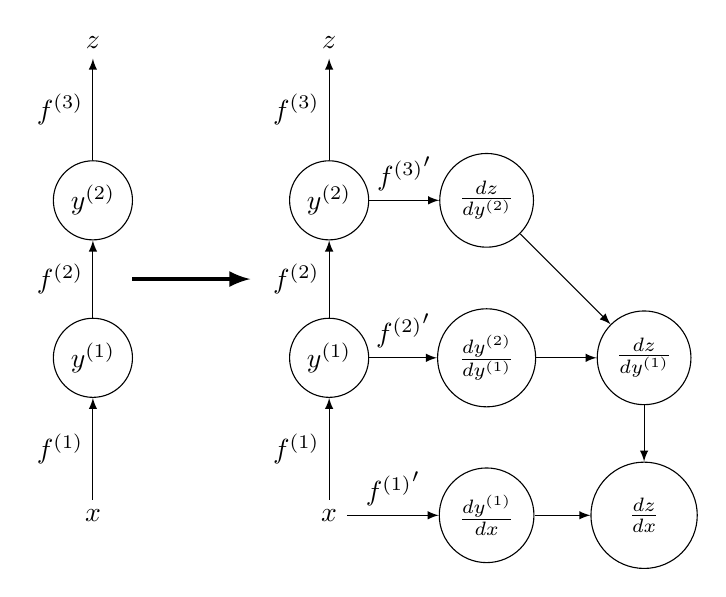
\begin{tikzpicture}
	\node[](layer0) at (0,0){$x$};
	\node[circle,draw](layer1) at (0,2){$y^{(1)}$};
	\draw[-latex](layer0.north)--(layer1)node[midway,left]{$f^{(1)}$};
	\node[circle,draw](layer2) at (0,4){$y^{(2)}$};
	\draw[-latex](layer1.north)--(layer2)node[midway,left]{$f^{(2)}$};
\node(output) at (0,6){$z$};
\draw[-latex](layer2)--(output)node[midway,left]{$f^{(3)}$};

\draw[-latex,ultra thick](0.5,3)--(2,3);

	\node[](2layer0) at (3,0){$x$};
	\node[circle,draw](2layer1) at (3,2){$y^{(1)}$};
	\draw[-latex](2layer0)--(2layer1)node[midway,left]{$f^{(1)}$};
	\node[circle,draw](2layer2) at (3,4){$y^{(2)}$};
	\draw[-latex](2layer1)--(2layer2)node[midway,left]{$f^{(2)}$};
\node(2output) at (3,6){$z$};
\draw[-latex](2layer2)--(2output)node[midway,left]{$f^{(3)}$};

\node[circle,draw](layer2dif)at (5,4){$\frac{dz}{dy^{(2)}}$};
\draw[-latex](2layer2)--(layer2dif)node[midway,above]{${f^{(3)}}'$};

\node[circle,draw](layer1dif)at (5,2){$\frac{dy^{(2)}}{dy^{(1)}}$};
\draw[-latex](2layer1)--(layer1dif)node[midway,above]{${f^{(2)}}'$};

\node[circle,draw](layer0dif)at (5,0){$\frac{dy^{(1)}}{dx}$};
\draw[-latex](2layer0)--(layer0dif)node[midway,above]{${f^{(1)}}'$};

\node[circle,draw](layer1nabla) at (7,2){$\frac{dz}{dy^{(1)}}$};
\draw[-latex](layer2dif)--(layer1nabla);
\draw[-latex](layer1dif)--(layer1nabla);

\node[circle,draw,minimum width=1.35cm](layer0nabla)at(7,0){$\frac{dz}{dx}$};
\draw[-latex](layer1nabla)--(layer0nabla);
\draw[-latex](layer0dif)--(layer0nabla);
\end{tikzpicture}
\end{figure}

\subsection{Adam optimizer}
\label{subsec:adam}
In the framework built for this thesis we use Adam (\textbf {Ada}ptive \textbf{m}oment estimation) optimizer (\cite{adam}). It is based on gradient descent, but it also conserves the momentum. In each learning step it uses a weighted average of previous gradients, thus it is not as dependent on the exact batch chosen for the step. It also helps overcome local minima, since it takes longer to reverse the direction of descent. It uses 4 parameters: $\alpha$ - learning rate, $\beta_1$ - gradient momentum decay, $\beta_2$ - second gradient moment momentum decay and $\epsilon$ - a small parameter to avoid division by zero. The description of algorithm can be found in Algorithm \autoref{alg:adam}. 
\begin{algorithm}[h]
\caption{Adam optimizer. This algorithm is exactly like it can be found in the original paper. $g_t^2$ denotes element-wise square. All vector operations are elemet-wise. $f_t$ represents the loss function $f$ realized over the training batch in the step $t$.}
\label{alg:adam}
\begin{algorithmic}
\REQUIRE $\alpha$: Stepsize
\REQUIRE $\beta_1, \beta_2 \in [0,1)$: Exponential decay rates for the moment estimates
\REQUIRE $f(\theta)$: Stochastic objective function with parameters $\theta$
\REQUIRE $\theta_0$: Initial parameter vector
\STATE $m_0 \leftarrow 0$ (Initialize $1^{\text{st}}$ moment vector)
\STATE $v_0 \leftarrow 0$ (Initialize $2^{\text{nd}}$ moment vector)
\STATE $t_0 \leftarrow 0$ (Initialize timestep)
\WHILE {$\theta_t$ not converged}
	\STATE $t\leftarrow t+1$
	\STATE $g_t \leftarrow \nabla_\theta f_t(\theta_{t-1})$ (Get gradients w.r.t. stochastic objective at timestep $t$)
	\STATE $m_t\leftarrow \beta_1\cdot m_{t-1}+(1-\beta_1)\cdot g_t$ (Update biased first moment estimate)
	\STATE $v_t\leftarrow \beta_2\cdot v_{t-1}+(1-\beta_2)\cdot g_t^2$ (Update biased second raw moment estimate)
	\STATE $\widehat{m_t}\leftarrow m_t/(1-\beta_1^t)$ (Compute bias-corrected first moment estimate)
	\STATE $\widehat{v_t}\leftarrow v_t/(1-\beta_2^t)$ (Compute bias-corrected second raw moment estimate)
	\STATE $\theta_t\leftarrow\theta_{t-1}-\alpha\cdot \widehat{m_t}/(\sqrt{\widehat{v_t}}+\epsilon)$ (Update parameters)
\ENDWHILE
\RETURN $\theta_t$ (Resulting parameters)
\end{algorithmic}
\end{algorithm}

The paper recommends using $\alpha = 0.001$, $\beta_1=0.9$, $\beta_2=0.999$ and $\epsilon=10^{-8}$. These values are also the default values in Tensorflow framework and were also used for building the models for this thesis.

This optimizer is best suited for very noisy functions or functions with a lot of local minima. In the step 7 of the loop we update each parameter with a different step size, dependent on the second moment. The effective step size for each element is $\Delta_t=\alpha\cdot\widehat{m_t}/\sqrt{\widehat{v_t}}$. Therefore the step size gets higher if the space is sparse, i.e. it only has several large gradients. If the gradients are closer to each other, we get smaller steps. We generally expect there to be a wild variance when we are further from the optimum (due to noise) that diminishes the closer we get. This way Adam can tune its step size based on how close we estimate that we are. 

In the $5^\text{th}$ and $6^\text{th}$ step of the loop we perform bias corrections. This is because the model without these corrections is naturally biased towards the initial value. As an example, let us assume that in the gradient $g_1$ has one element value $10$. Then $m_1$ has for this element $10\cdot(1-\beta_1)$, that is $1$ if we use recommended parameters. The average, however, should obviously be $10$. If we do the correction, this is exactly what we have.

Another nice property of Adam is its invariance towards rescaling. If we rescale the gradients with a positive constant $c$, it cancels out: $\Delta_t = c\cdot\widehat{m_t}/\sqrt{\widehat{v_t}\cdot c^2}=\widehat{m_t}/\sqrt{\widehat{v_t}}$.

More information about this algorithm, including the convergence analysis, proof of convergence or extensions can be found in the original paper.